\chapter{วิธีการตรวจสอบตราของแสตมป์ที่นำเสนอ}
\label{ch:proposed}
ในบทนี้จะเป็นการอธิบายวิธีการตรวจสอบตราของแสตมป์สุราโดยอัตโนมัติที่นำเสนอในโครงงานวิจัยนี้  โดยวิธีการที่นำเสนอใช้วิธีการทางการประมวลผลภาพ  ในหัวข้อ 3.1 จะเป็นการอธิบายโครงสร้างของระบบเพื่อใช้ในการถ่ายภาพ หัวข้อ 3.2 อธิบายแนวคิดและภาพรวมของวิธีที่นำเสนอ ซึ่งประกอบไปด้วย 2 ขั้นตอนหลักคือการตัดภาพรูปนกวายุภักษ์ และการนำภาพรูปนกวายุภักษ์ ไปตรวจสอบว่าเป็นแสตมป์แท้หรือปลอม ซึ่งจะอธิบายแต่ละส่วนนี้ในหัวข้อ 3.3 และ 3.4 ตามลำดับ
\section{โครงสร้างระบบเพื่อใช้ในการถ่ายภาพของแสตมป์}
ระบบตรวจสอบแสตมป์อัตโนมัติที่นำเสนอใช้วิธีการทางการประมวลผลภาพ ดังนั้นการถ่ายภาพจึงมีความสำคัญกับวิธีที่จะนำเสนอ โดยสำหรับในโครงงานวิจัยนี้ ได้กำหนดระบบการถ่ายภาพไว้ดังรูปที่~\ref{fig:hardware}

\begin{figure}[!ht]
\centering
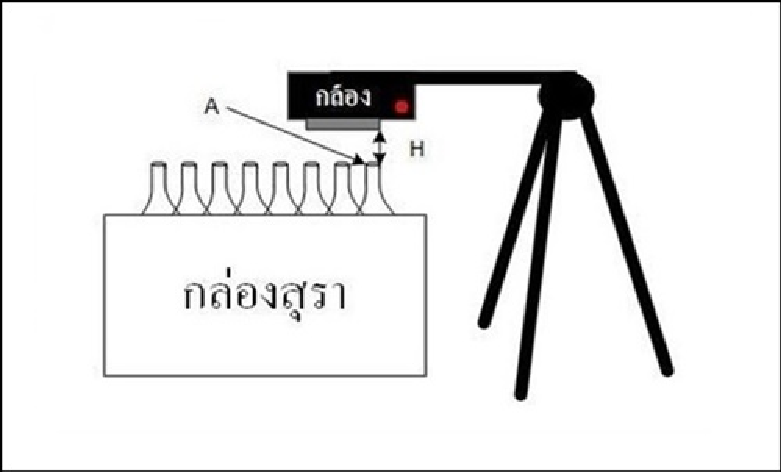
\includegraphics[width=0.9\textwidth]{capture-hardware}
\caption{โครงสร้างทางฮาร์ดแวร์ของระบบการคัดแยกตราของแสตมป์}
\label{fig:hardware}
\end{figure}

เนื่องจากแสตมป์เครื่องดื่มที่มีแอลกอฮอร์จะถูกกำหนดไว้ให้ติดไว้ที่บริเวณฝาผิดของขวด จึงได้กำหนดวิธีการถ่ายภาพไว้ให้เป็นการถ่ายจากด้านบน ด้วยกล้องถ่ายภาพสี ในพื้นที่ที่มีแสงเพียงพอ  ด้วยความสูงจากบริเวณแสตมป์ที่เหมาะสม การถ่ายภาพจะต้องให้ได้ภาพของตรานกวายุภักษ์ ที่อยู่ในแสตมป์ ดังตัวอย่างในรูปที่~\ref{fig:stamp-real} และ~\ref{fig:stamp-fake}  สำหรับกรณีแสตมป์จริงและแสตมป์ปลอมตามลำดับ

\begin{figure}[!ht]
\centering
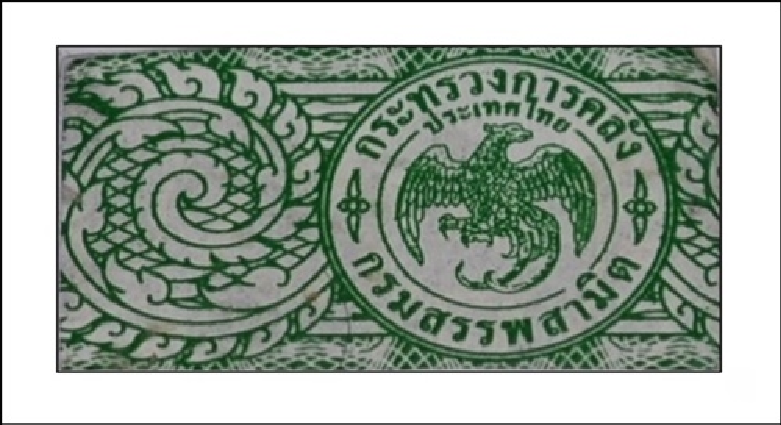
\includegraphics[width=0.9\textwidth]{sample-stamp-real}
\vspace{2em}
\caption{ตัวอย่างรูปของแสตมป์จริงบริเวณตรานกวายุภักษ์ ที่ได้จากการถ่ายภาพ}
\label{fig:stamp-real}
\end{figure}

\begin{figure}[!ht]
\centering
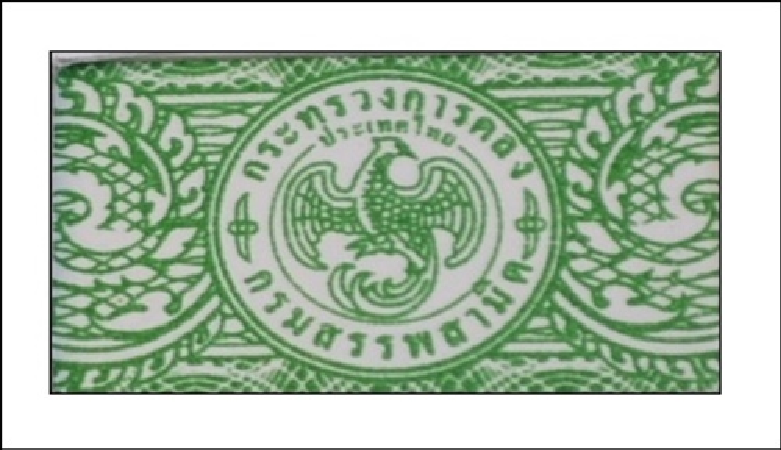
\includegraphics[width=0.9\textwidth]{sample-stamp-fake}
\vspace{2em}
\caption{ตัวอย่างรูปของแสตมป์ปลอมบริเวณตรานกวายุภักษ์ ที่ได้จากการถ่ายภาพ}
\label{fig:stamp-fake}
\end{figure}

\section{แนวคิดของวิธีการตรวจสอบที่นำเสนอ}
จากการพิจารณารูปแสตมป์ตัวอย่างที่ถ่ายมาจำนวนหนึ่ง พบว่าลักษณะเด่นที่แตกต่างกันระหว่างแสตมป์จริงและแสตมป์ปลอมจะเกิดขึ้นบริเวณตรานกวายุภักษ์ โดยลักษณะที่เด่นที่สุดของความแตกต่างคือความเข้มของสีบริเวณตรานกวายุภักษ์  ดังแสดงในรูปที่~\ref{fig:stamp-real}  ซึ่งเป็นตัวอย่างรูปของแสตมป์จริง และ รูปที่~\ref{fig:stamp-fake}  ซึ่งเป็นตัวอย่างรูปของแสตมป์ปลอม จากข้อสังเกตดังกล่าวโครงงานวิจัยนี้จึงได้นำเสนอแนวคิดในการตรวจสอบแสตมป์ดังนี้

ในขั้นแรกของวิธีการคือ การตัดเอาเฉพาะส่วนของบริเวณตรานกวายุภักษ์ ออกมา ซึ่งเนื่องจากบริเวณตรานกวายุภักษ์ จะถูกล้อมรอบไว้ด้วยวงกลม โครงงานวิจัยนี้จึงมีแนวคิดในการนำเอาวิธีการทางการแปลงแบบวงกลมฮัฟ (Circle Hough Transform)  มาใช้ในการตัดเอาบริเวณตรานกวายุภักษ์ออกมา โดยจากการทดลองหลายครั้ง ทำให้ขนาดรัศมีวงกลมของตรานกวายุภักษ์ที่อยู่ในแสตมป์สุราว่าอยู่ในช่วงใด  เราจึงสามารถใช้วิธีการแปลงฮัฟวงกลมในการค้นหาวงกลมที่มีรัศมีอยู่ในช่วงดังกล่าวได้ โดยการเลือกเพียงวงกลมเดียวมา เพราะในภาพแสตมป์ที่ถ่ายมาจะมีตรานกวายุภักษ์เพียงตราเดียว รูปที่~\ref{fig:sample-hough} แสดงรูปตัวอย่างของผลของการใช้การแปลงฮัฟวงกลมในการค้นหาตรานกวายุภักษ์  และรูปที่~\ref{fig:sample-bird-cut} แสดงภาพที่ตัดเฉพาะส่วนที่เป็นนกวายุภักษ์ออกมาโดยการเลือกเอาเฉพาะภาพที่อยู่ภายในวงของวงกลมที่ได้จากการแปลงฮัฟวงกลม


\begin{figure}[!ht]
\centering
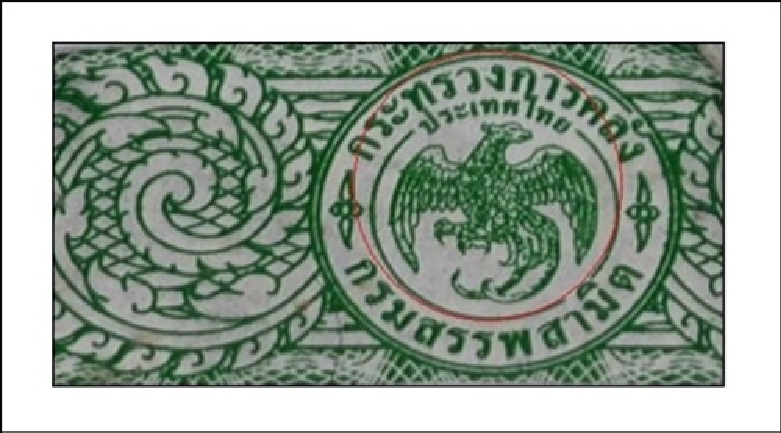
\includegraphics[width=0.9\textwidth]{sample-hough}
\vspace{2em}
\caption{ตัวอย่างผลของการใช้การแปลงฮัฟวงกลมแสดงด้วยเส้นสีแดงเพื่อค้นหาตรานกวายุภักษ์}
\label{fig:sample-hough}
\end{figure}

\begin{figure}[!ht]
\centering
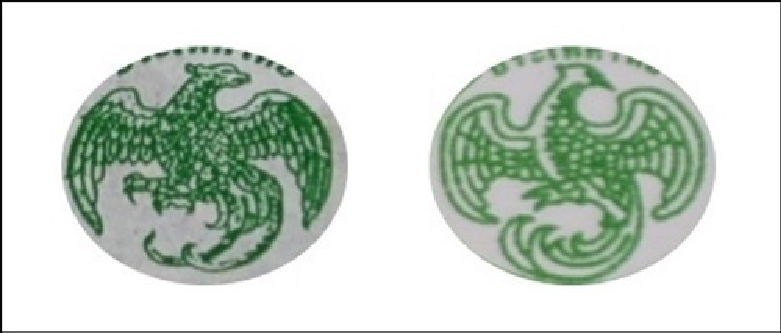
\includegraphics[width=0.9\textwidth]{sample-bird-cut}
\vspace{2em}
\caption{รูปตัวอย่างของตรานกวายุภักษ์ที่ตัดจากภาพของแสตมป์โดยการตัดเอาเฉพาะส่วนที่อยู่ในวงกลมที่ได้จากการแปลงฮัฟวงกลม}
\label{fig:bird-cut}
\end{figure}


%\begin{figure}[!ht]
%\centering
%\includegraphics[width=0.9\textwidth]{355.jpg}
%\vspace{2em}
%\caption{ฮิสโตแกรมของรูปนกวายุภักษ์จากแสตมป์ปลอม}
%\label{fig:355}
%\end{figure}

\begin{figure}[!]
\centering
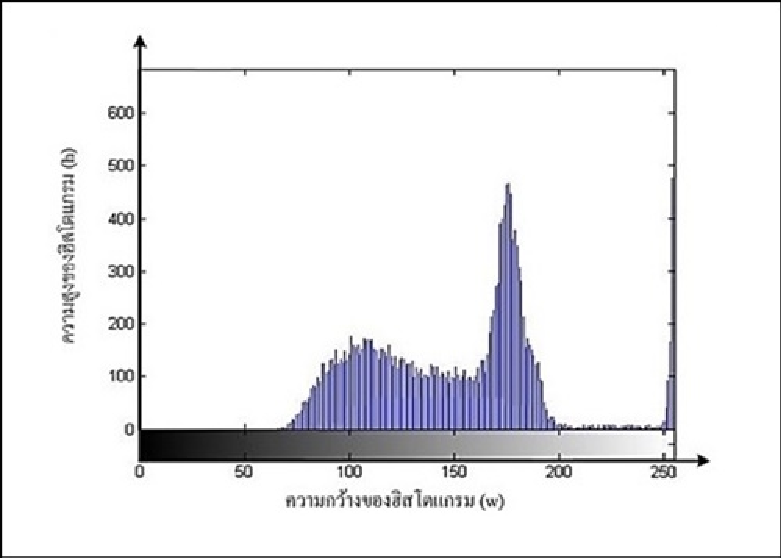
\includegraphics[width=0.81\textwidth]{histogram-real}
\vspace{2em}
\caption{ฮิสโตแกรมของรูปนกวายุภักษ์ที่ตัดมาจากแสตมป์จริง}
\label{fig:histogram-real}
\end{figure}
\begin{figure}[!]
\centering
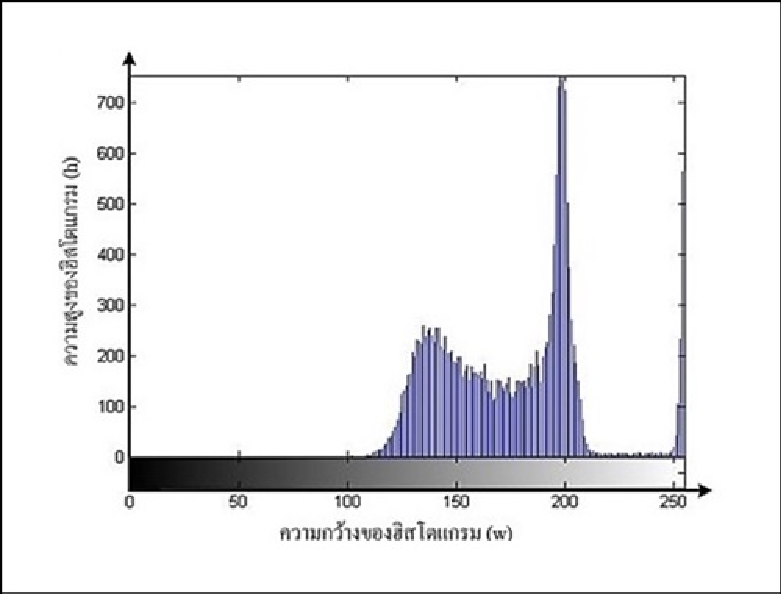
\includegraphics[width=0.81\textwidth]{histogram-fake}
\vspace{2em}
\caption{ฮิสโตแกรมของรูปนกวายุภักษ์ที่ตัดมาจากแสตมป์ปลอม}
\label{fig:histogram-fake}
\end{figure}

เมื่อสังเกตตรานกวายุภักษ์ ที่ตัดออกมาจากแสตมป์จริงและแสตมป์ปลอม จะพบว่าตรานกวายุภักษ์ ของแสตมป์จริงจะมีความเข้มมากกว่า และมีรายละเอียดมากกว่า เช่น บริเล็ปของนกในตราของจริงจะมีความชัดเจนมากกว่า คำถามของเราคือจะใช้วิธีการทางการประมวลผลภาพอะไรสำหรับการตรวจสอบความแตกต่างดังกล่าว  แนวคิดที่นำมาใช้ในโครงงานวิจัยนี้คือ ลองพิจารณาจากใช้วิธีที่ง่ายก่อน  ถ้าไม่ได้จึงพิจารณาใช้วิธีที่ยากซับซ้อนขึ้น

เนื่องจากความแตกต่างที่ชัดเจนคือความเข้มสี ดังนั้นจึงมีความเป็นไปได้ที่ฮิสโตแกรม (histogram) ของภาพตรานกวายุภักษ์จริงและภาพตรานกวายุภักษ์ปลอม จะบอกความแตกต่างได้  เนื่องจากสีที่ใช้พิมพ์แสตมป์เป็นสีเขียว จึงตัดเอาเฉพาะส่วนของสีเขียวไปสร้างฮิสโตแกรมดังแสดงในรูปที่~\ref{fig:histogram-real} และ~\ref{fig:histogram-fake}  สำหรับตรานกวายุภักษ์จริงและปลอมตามลำดับ จากการเปรียบเทียบคุณลักษณะเด่นของฮิสโตแกรม ของภาพส่วนสีเขียวของตรานกวายุภักษ์ของแสตมป์จริงและของแสตมป์ปลอม  พบว่าลักษณะของการกระจายของอิสโตแกรมคล้ายคลึงกัน กล่าวคือจะมีพื้นที่ของการกระจายของความเข้มสีเขียวอย่างต่อเนื่องกัน แต่มีลักษณะเด่นของฮิสโตแกรม 2 ประการที่แตกต่างกันคือ
\begin{enumerate}
\item ความกว้างของฮิสโตแกรมในส่วนที่ต่อเนื่องกัน ซึ่งพบว่าความกว้างของฮิสโตแกรมของตรานกวายุภักษ์ของแสตมป์จริงจะมากกว่า ของตรานกวายุภักษ์ของแสตมป์ปลอม สำหรับในโครงงานวิจัยนี้เราจะใช้สัญลักษณ์ $w$ แทนความกว้างของอิสโตแกรมดังกล่าวนี้
\item ความสูงที่สูงที่สุดของฮิสโตแกรมในส่วนที่ต่อเนื่องกัน ซึ่งพบว่าความสูงของอิสโตแกรมของตรา
นกวายุภักษ์ จากแสตมป์จริงจะมากกว่า ของตรานกวายุภักษ์ จากแสตมป์ปลอม สำหรับในโครงงานวิจัยนี้เราจะใช้สัญลักษณ์ $h$ แทนความสูงของอิสโตแกรมดังกล่าวนี้
\end{enumerate}

ด้วยคุณลักษณะของฮิสโตแกรมที่แตกต่างกัน 2 ข้อดังกล่าว เราสามารถนำไปใช้เป็นลักษณะเด่นในการคัดแยกว่าแสตมป์เป็นของจริงหรือปลอมได้ วิธีการคัดแยกที่นำมาใช้ในโครงงานศึกษาวิจัยนี้ เป็นวิธีการนำเอาลักษณะเด่นทั้งสองคือ ความกว้างของฮิสโตแกรม ($w$) และ ความสูงของฮิสโตแกรม ($h$) ไปพล็อตเป็นคู่พิกัด $(w, h)$ บนระนาบโดย $w$ เป็นแกน $x$ และ $h$ เป็นแกน $y$ แล้วใช้เส้นตรงบนระนาบดังกล่าวเป็นเส้นแบ่งกลุ่มของจริงกับของปลอม

จากแนวคิดของการแก้ปัญหาวิจัยดังกล่าว เราจะได้ภาพรวมของขั้นตอนการตรวจสอบแสตมป์ที่นำเสนอในโครงงานศึกษาวิจัยนี้ตามบล็อกไดอะแกรม (block diagram) ดังรูปที่~\ref{fig:block-diagram} โดยรายละเอียดของขั้นตอนการตัดเอาเฉพาะตรานกวายุภักษ์และการคัดแยกจะอธิบายไว้ในหัวข้อ~\ref{sec:bird-cut-method}~และ~\ref{sec:classification} ตามลำดับ

\begin{figure}[!ht]
\centering
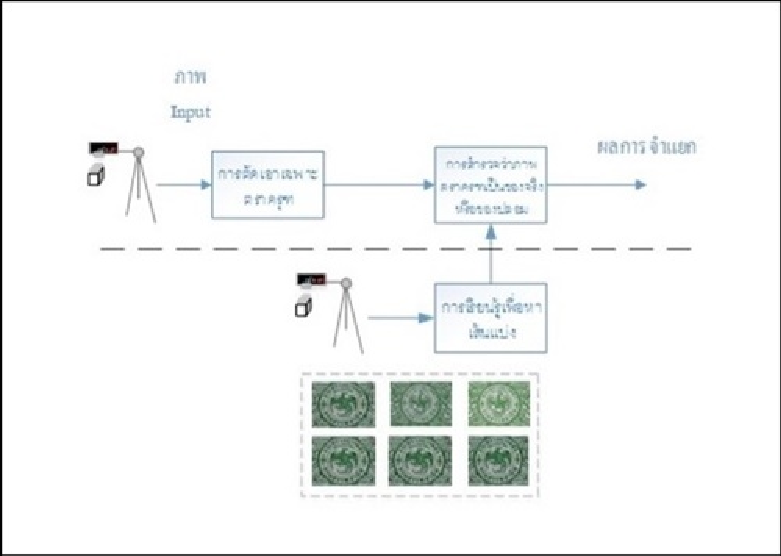
\includegraphics[width=0.9\textwidth]{block-diagram}
\vspace{2em}
\caption{บล็อกไดอะแกรมของวิธีการตรวจสอบแสตมป์อัตโนมัติ}
\label{fig:block-diagram}
\end{figure}


\section{วิธีการตัดเอาเฉพาะภาพตรานกวายุภักษ์}
\label{sec:bird-cut-method}
ตามที่ได้กล่าวไว้ในแนวคิดของการแก้ปัญหาแล้วว่าโครงงานวิจัยนี้ได้นำวิธีการแปลงแบบฮัฟ มาใช้เป็นเครื่องมือในการค้นหาวงกลมที่ล้อมรอบตรานกวายุภักษ์ที่อยู่ในแสตมป์ หัวข้อนี้อธิบายขั้นตอนการตัดเอาภาพตรานกวายุภักษ์ ดังกล่าวดังนี้

\begin{figure}[!ht]
\centering
\vspace{2em}
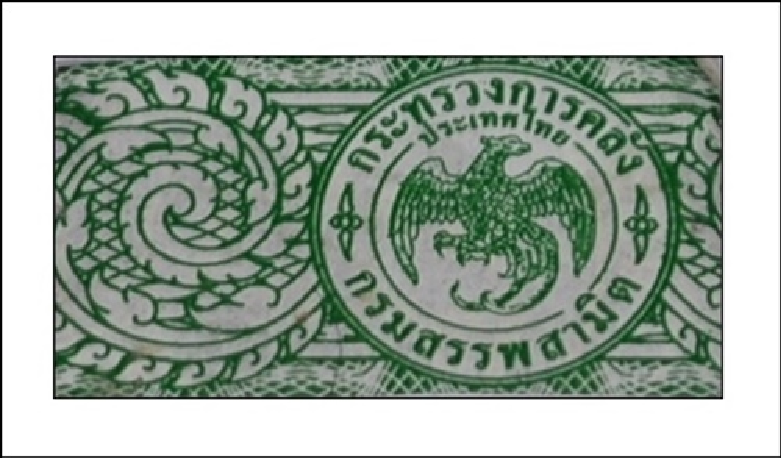
\includegraphics[width=0.9\textwidth]{input-image}
\vspace{2em}
\caption{ภาพของแสตมป์ที่ต้องการตรวจสอบ นำเข้าในโปรแกรมเพื่อการตัดเอาส่วนของตรานกวายุภักษ์}
\label{fig:input-image}
\end{figure}

\begin{figure}[!ht]
\centering
\vspace{2em}
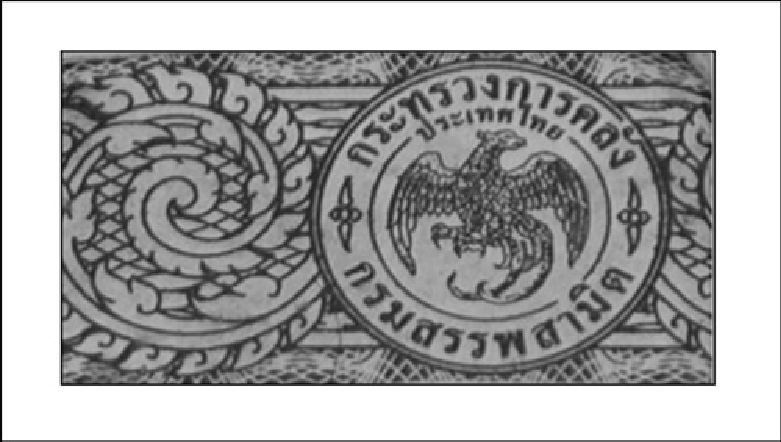
\includegraphics[width=0.9\textwidth]{grey-image}
\vspace{2em}
\caption{ภาพระดับสีเทาของภาพแสตมป์ในรูปที่~\ref{fig:input-image}}
\label{fig:grey}
\end{figure}

%\begin{itemize}

\textbf{ขั้นตอนที่ 1:} นำเข้าภาพแสตมป์ รูปที่~\ref{fig:input-image} แสดงภาพตัวอย่างของภาพแสตมป์ที่นำเข้าสู่กระบวนการ สังเกตว่าภาพอินพุทนี้มีการตัดเอาเฉพาะส่วนที่มีตราแสตมป์เท่านั้น ในโครงงานศึกษาวิจัยนี้เราจะสมมุติว่ามีระบบตัดภาพนี้ให้แล้ว

\textbf{ขั้นตอนที่ 2:} แปลงภาพจากขั้นตอนที่ 1 เป็นภาพระดับเทา รูปที่~\ref{fig:grey} แสดงผลของขั้นตอนนี้เมื่อใช้กับภาพตัวอย่างในรูปที่~\ref{fig:input-image}

\textbf{ขั้นตอนที่ 3:} แปลงภาพระดับเทาเป็นภาพขาวดำ รูปที่~\ref{fig:bw} แสดงผลของขั้นตอนนี้เมื่อใช้กับภาพระดับสีเทานรูปที่~\ref{fig:bw}

\textbf{ขั้นตอนที่ 4:} ใช้วิธีการหาเส้นขอบด้วยวิธี canny เพื่อการหาขอบ  โดยอินพุทเป็นภาพขาวดำจากขั้นตอนที่ 3 เพราะต้องการลดจำนวนจุดขาวของภาพลงไป รูปที่~\ref{fig:edge} เป็นผลของการหาขอบของภาพในรูปที่~\ref{fig:bw} 

\begin{figure}[!]
\centering
\vspace{2em}
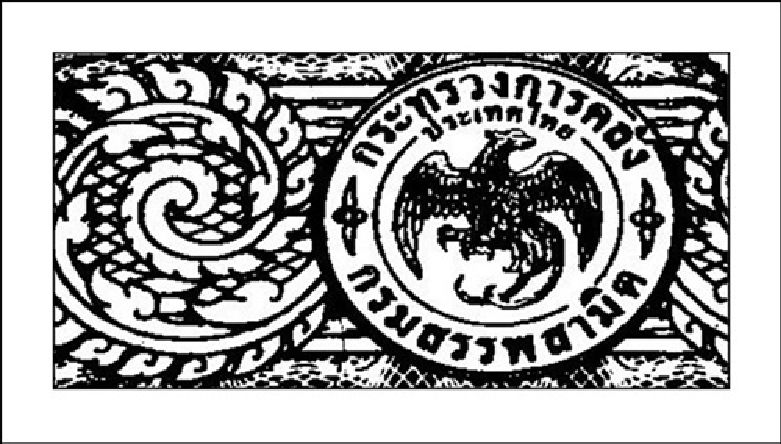
\includegraphics[width=0.9\textwidth]{bw-image}
\vspace{2em}
\caption{ภาพขาวดำที่ได้จากการแปลงภาพระดับสีเทาของแสตมป์จากรูปที่~\ref{fig:grey}}
\label{fig:bw}
\end{figure}


\begin{figure}[!]
\centering
\vspace{2em}
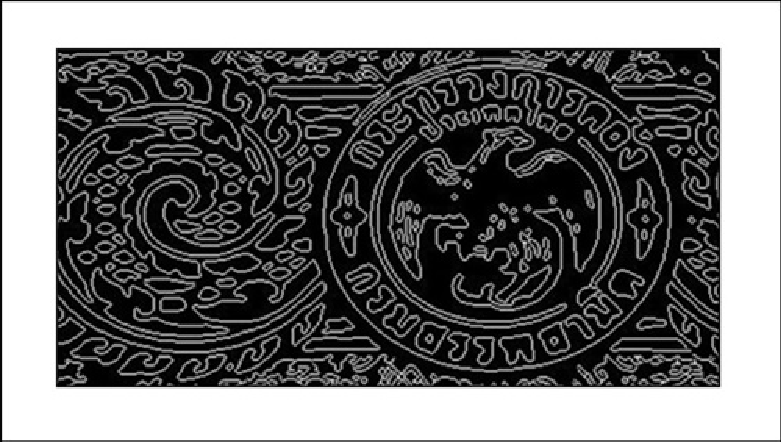
\includegraphics[width=0.9\textwidth]{edge-image}
\vspace{2em}
\caption{ภาพที่ได้จากการหาเส้นขอบด้วยวิธี canny ของภาพตัวอย่างดังรูปที่~\ref{fig:bw}}
\label{fig:edge}
\end{figure}


\begin{figure}[!]
\centering
\vspace{2em}
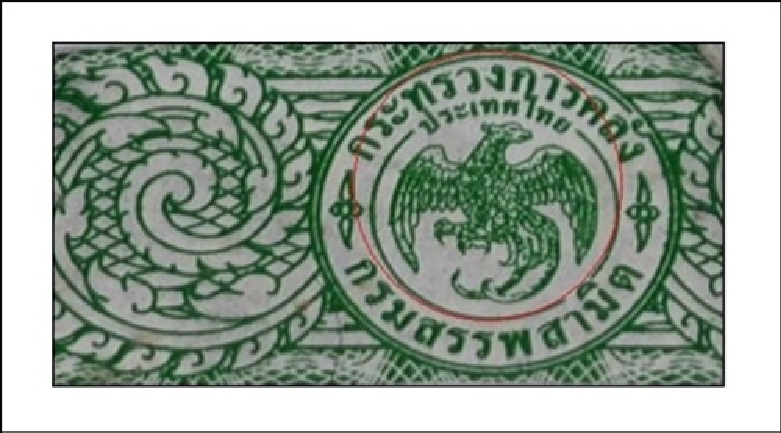
\includegraphics[width=0.9\textwidth]{hough-result}
\vspace{2em}
\caption{ตัวอย่างผลลัพธ์ของการค้นหาวงกลมของภาพตัวอย่างในรูปที่~\ref{fig:input-image} ด้วยการใช้การแปลงฮัฟวงกลม}
\label{fig:hough-result}
\end{figure}


\begin{figure}[!]
\centering
\vspace{2em}
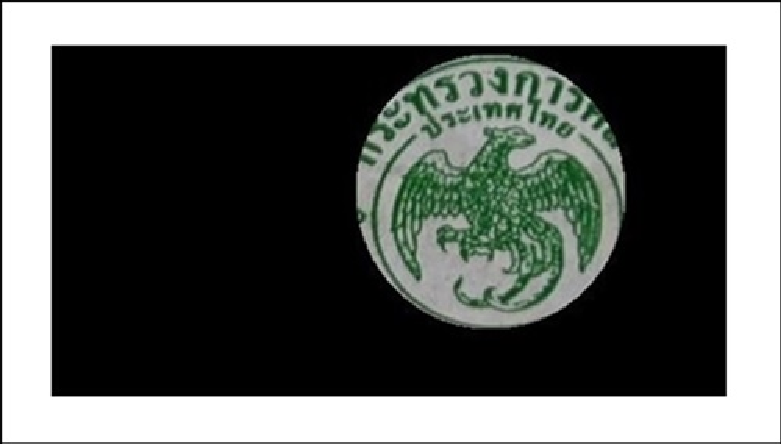
\includegraphics[width=0.9\textwidth]{bird-cut-image}
\vspace{2em}
\caption{ตัวอย่างผลของการตัดภาพอินพุทเพื่อเอาเฉพาะส่วนของภายในวงกลมที่ได้จากขั้นตอนที่ 6}
\label{fig:bird-cut-sample}
\end{figure}



\textbf{ขั้นตอนที่ 5:} ใช้การแปลงแบบฮัฟวงกลม (Circle Hough Transform) เพื่อสร้าง  Hough Space  ของวงกลมที่มีรัศมีในช่วงที่ครอบคลุม โดยใช้ขนาดของรัศมีวงนอกสุดของกรอบวงกลมที่ล้อมรอบตรานกวายุภักษ์เป็นขอบเขตสูงสุด

\textbf{ขั้นตอนที่ 6:} เลือกวงกลมจาก Hough Space ในขั้นตอนที่ 5 ที่มีความถี่ของการเกิดมากที่สุด ผลที่ได้ในขั้นนี้จะอยู่ในรูปของตำแหน่งจุดศูนย์กลางและรัศมี รูปที่~\ref{fig:hough-result} แสดงผลของวงกลมที่ได้จากภาพของแสตมป์ตัวอย่างดังรูปที่~\ref{fig:input-image}

\textbf{ขั้นตอนที่ 7:} ตัดเอาเฉพาะส่วนของภาพอินพุทที่อยู่ภายในวงกลมที่ได้ในขั้นตอนที่ 6 รูปที่~\ref{fig:bird-cut-sample} แสดงภาพของการตัดสำหรับกรณีภาพตัวอย่างตามรูปที่~\ref{fig:input-image}
%\end{itemize}



%\begin{figure}[!ht]
%\centering
%\vspace{2em}
%\includegraphics[width=0.9\textwidth]{3-13}
%\vspace{2em}
%\caption{ภาพต้นฉบับเพื่อหาระยะความสูงของผู้ใช้บริการ และ กระบวนการประมวลผลภาพทำการคำนวณหาระยะความสูง แล้วส่งคำสั่งให้ชุดบอร์ดมอเตอร์ควบคุมระบบชุดรับภาพเอกซเรย์}
%\label{fig:3-13}
%\end{figure}

\section{วิธีการแยกแยะตรานกวายุภักษ์}
\label{sec:classification}
ตามที่ได้กล่าวไว้ในแนวคิดของการแก้ปัญหา ในโครงงานศึกษาวิจัยนี้  จะใช้คุณสมบัติเด่นของฮิสโตแกรมของภาพตรานกวายุภักษ์ ที่ได้จากการตัดด้วยวิธีที่นำเสนอตามหัวข้อที่~\ref{sec:bird-cut-method} เพื่อการตรวจสอบว่าแสตปม์นั้นเป็นของจริงหรือปลอม จากแนวคิดที่นำเสนอพบว่าคุณลักษณะ 2 ตัวของฮิสโตแกรมดังแสดงในรูปที่~\ref{fig:feature-def} ที่สามารถใช้ในการแยกแยะตราวายุภักษ์ของแสตมป์จริงกับของแสตมป์ปลอมออกจากกันคือ
\begin{enumerate}
\item ความสูงของฮิสโตแกรมของภาพตรานกวายุภักษ์ แทนด้วย $h$ เป็นค่าความถี่ที่ปรับให้อยู่ระหว่าง 0 ถึง 1 ที่มีค่าสูงสุด
\item ความกว้างของฮิสโตแกรมของภาพตรานกวายุภักษ์ แทนด้วย $w$ เป็นค่าความกว้างของฮิสโตแกรมทีมีความถี่มากกว่า 20/
\end{enumerate}

\begin{figure}[!ht]
\centering
\vspace{2em}
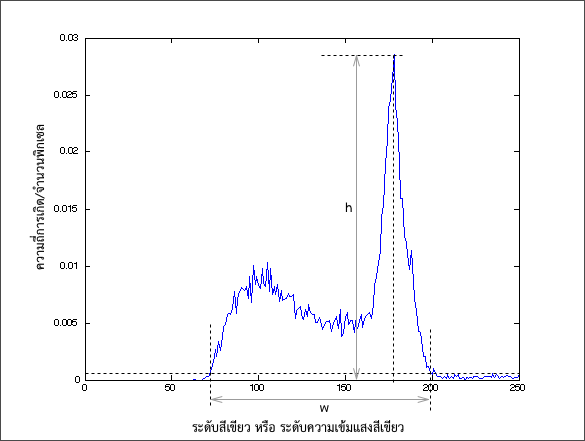
\includegraphics[width=0.9\textwidth]{historgram-norm}
\vspace{2em}
\caption{นิยามของค่า $w$ และ $h$  ที่ใช้เป็นลักษณะเด่นในการแยกแยะตรานกวายุภักษ์}
\label{fig:feature-def}
\end{figure}

วิธีการแยกแยะที่นำมาใช้ เป็นวิธีการใช้เส้นเบ่งแบบเส้นตรง (linear classification line) ของจุดพิกัด $(w,h)$ โดยจุดพิกัดที่ได้จากตราวายุภักษ์ของแสตมป์จริงจะอยู่ข้างล่างของเส้นแบ่ง เพราะฮิสโตแกรมของมันจะมีค่า $h$  (แกน $y$) ที่ต่ำของปลอม ในขณะที่ $w$ (แกน $x$) ของตราวายุภักษณ์ของจริงจะมีค่ามากกว่าของตราวายุภักษ์ปลอม  เส้นแบ่งดังกล่าวจะใช้วิธีการเรียนรู้ซี่งอธิบายในหัวข้อ~\ref{sec:training} 

วิธีการแยกแยะตราวายุภักษณ์ที่นำมีขั้นตอนดังนี้

\textbf{ขั้นตอนที่ 1:} นำเข้าภาพตรานกวายุภักษ์ ที่ได้จากขั้นตอนการตัดภาพตรานกวายุภักษ์ดังตัวอย่างในรูปที่~\ref{fig:bird-cut-sample} ไปหาฮิสโตแกรมของระดับสีเขียว ได้ผลลัพธ์ดังตัวอย่างในรูปที่~\ref{fig:histogram-example}

\textbf{ขั้นตอนที่ 2:} ปรับความถี่ของฮิสโตแกรมให้เป็นค่าระหว่าง 0 ถึง 1 โดยการหารด้วยจำนวนจุดของภาพ

\textbf{ขั้นตอนที่  3:} ตัดฮิสโตแกรมให้เหลือเฉพาะส่วนของ Bin  จาก 21 ถึง 250 เพื่อให้ใต้เฉพาะส่วนของฮิสโตแกรมที่ต่อเนื่อง 

\textbf{ขั้นตอนที่ 4:} หาความสูง $h$ ได้โดยการหาค่าที่มากที่สุดของกราฟอิสโตแกรมจากขั้นตอนที่ 3

\textbf{ขั้นตอนที่ 5:} หาความกว้าง $w$ ตามนิยามตามรูปที่~\ref{fig:feature-def}

\textbf{ขั้นตอนที่ 6:} ถ้า $(w,h)$ อยู่ใต้เส้นแบ่งแสดงว่าเป็นภาพตรานกวายุภักษ์อินพุทเป็นของแสตมป์จริง ถ้าไม่เช่นนั้นแสดงว่าเป็นของแสตมป์ปลอม

%\begin{figure}[!ht]
%\centering
%\vspace{2em}
%\includegraphics[width=0.9\textwidth]{3-13}
%\vspace{2em}
%\caption{ภาพต้นฉบับเพื่อหาระยะความสูงของผู้ใช้บริการ และ กระบวนการประมวลผลภาพทำการคำนวณหาระยะความสูง แล้วส่งคำสั่งให้ชุดบอร์ดมอเตอร์ควบคุมระบบชุดรับภาพเอกซเรย์}
%\label{fig:3-13}
%\end{figure}


\begin{figure}[!ht]
\centering
\vspace{2em}
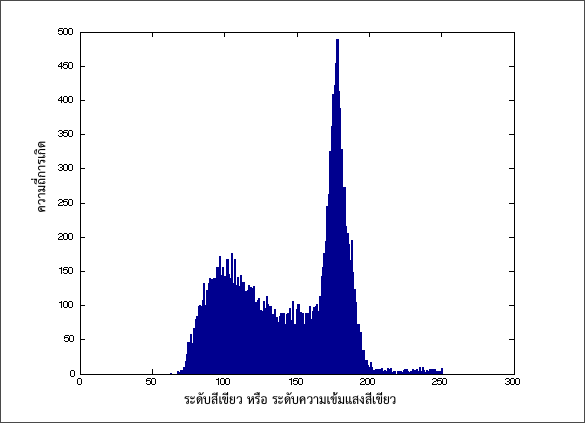
\includegraphics[width=0.9\textwidth]{histogram-example-stamp}
\vspace{2em}
\caption{ตัวอย่างอิสโตแกรมของภาพระดับสีเขียวของตรานกวายุภักษ์จากรูปที่~\ref{fig:bird-cut-sample}}
\label{fig:histogram-example}
\end{figure}

\begin{figure}[!hb]
\centering
\vspace{2em}
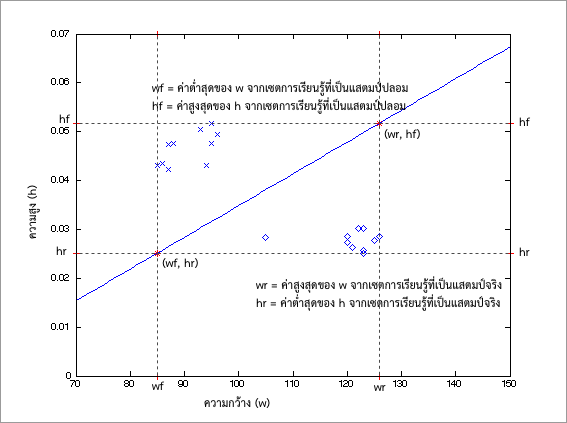
\includegraphics[width=0.81\textwidth]{training-method}
\vspace{2em}
\caption{เส้นตรงสำหรับการแยกแยะที่ได้จากการเรียนรู้ด้วยภาพแสตมป์จริงและแสตมป์ปลอมอย่างละ 5 ภาพ ($n=5$)}
\label{fig:training-result}
\end{figure}

\section{การเรียนรู้เพื่อหาเส้นแบ่งการคัดแยก}
\label{sec:training}
เส้นตรงที่ใช้ในการตัดสินว่าภาพตรานกวายุภักษ์เป็นของแสตมป์จริงหรือปลอมหาได้จากการเรียนรู้โดยมีขั้นตอนดังต่อไปนี้

\begin{enumerate}
\item เลือกเซตของภาพที่ใช้ในการเรียนรู้  โดยใช้ภาพจากแสตมป์จริงและแสตมป์ปลอมจำนวน $n$ ภาพเท่ากัน   ให้ $r_1, r_2,\ldots r_n$ เป็นภาพตรานกวายุภักษ์ที่ตัดจากแสตมป์จริงจำนวน $n$ ภาพ และให้ $f_1, f_2,\ldots , f_n$ เป็นภาพตรานกวายุภักษ์ที่ตัดจากแสตมป์ปลอมจำนวน $n$ ภาพ
\item ใช้วิธีการตัดตราวายุภักษ์ที่เสนอในหัวข้อ~\ref{sec:bird-cut-method}  ในการตัดภาพวายุภักษณ์ของภาพที่ใช้ในการเรียนรู้ทั้งหมด
\item ใช้วิธีการหาค่า $w$ และ $h$ ของตราวายุภักษณ์ที่ตัดมาทุกอัน โดยให้ $w_r(i)$ และ $h_r(i)$ เป็นค่า $w$ และ $h$ ของภาพในการเรียนรู้ที่เป็นแสตมป์จริงลำดับที่ $i$ และให้ $w_f(i)$ และ $h_f(i)$ เป็นค่า $w$ และ $h$ ของภาพในการเรียนรู้ที่เป็นแสตมป์ปลอมลำดับที่ $i$, $i = 1, 2,\ldots n$
\item หาเส้นตรงที่เป็นเส้นแบ่งกลุ่มของ $(w_r(i), h_r(i))$ ออกจากกลุ่มของ $(w_f(i), h_f(i))$ 
\begin{itemize}
\item เลือกมุมซ้ายล่างของกลุ่ม $(w_{min}, h_{min})$ และจุดมุมขวาของกลุ่ม $(w_{max}, h_{max})$ โดยที่
\begin{itemize}
\item $w_{min}$ เป็นค่าน้อยที่สุดของ   $w_f$ 
\item $h_{min}$ เป็นค่าน้อยที่สุดของ $h_r$ 
\item $w_{max}$ เป็นค่าน้อยที่สุดของ   $w_r$ 
\item $h_{max}$ เป็นค่าน้อยที่สุดของ $h_f$ 
\end{itemize}
\item เลือกเส้นแบ่งเป็นเส้นตรงจากจุด $(w_{min},h_{min})$ ซึ่งเป็นจุดด้านมุมซ้ายล่างกับจุด $(w_{max}, h_{max})$ ซึ่งเป็นจุดมุมขวาบน
\end{itemize}
\end{enumerate}
 
 รูปที่~\ref{fig:training-result} แสดงตัวอย่างของผลการเรียนรู้ด้วย $n=10$



